\chapter{Iteracion 5: Diseño final del Software} % (fold)
\label{cha:iteracion_5}

\section{Introduccion} % (fold)
\label{sec:introduccion}

% section introduccion (end)

\section{Requerimientos de la iteracion} % (fold)
\label{sec:requerimientos_de_la_iteracion}

\begin{itemize}
\item
\end{itemize}


% section requerimientos_de_la_iteracion (end)

\section{Desarrollo} % (fold)
\label{sec:desarrollo}

\subsection{Logica para permitir intervalos individuales de medicion: Buffer de conversion estatico y dinamico} % (fold)
\label{sub:logica_para_permitir_intervalos_individuales_de_medicion_buffer_de_conversion_estatico_y_dinamico}

En esta seccion, ocupamos el rediseño de las funciones del conversor con el objetivo de lograr que el usuario pueda configurar tiempos de intervalos de mediciones en cada canal por separado. El tiempo entre cada medicion no es menor, dado que dependiendo el tipo de sensor, puede necesitarse que las mediciones sean de frecuencia alta o baja.

En la seccion \ref{sub:logica_de_las_funciones_del_conversor}, se explica el funcionamiento del buffer del conversor. Este buffer posee 8 posiciones, una por cada canal, con el objetivo de informar al programa el estado de ese canal. Estos estados son: inhabilitado, canal unico, diferencial.

En esta version, se utilizan dos buffers de 11 posiciones cada uno. Cada posicion ya no representa un unico canal sino que representa una via de conversion. Elaboraremos esto mas adelante. Estos buffers pueden diferenciarse uno del otro en que uno puede decirse que es "estatico", y el otro "dinamico". De la misma manera que el buffer original, el buffer estatico determina si un canal esta habilitado o no: Si la posicion que corresponde a ese canal contiene un 0, entonces ese canal esta habilitado. Cualquier numero distinto de 0 indica que el canal esta habilitado. A diferencia del buffer original, el modo de conversion ya no se identifica con un numero, sino con la posicion dentro del buffer, ya sea estatico o dinamico. Las posiciones del 0 al 7 estan reservadas para los 8 canales del conversor en modo canal unico, y las posiciones del 8 al 11 son para el modo diferencial. 
El contenido de cada elemento en el buffer es un numero que va de 1 a 255, en el caso en que este habilitado. Ese numero representa el tiempo que existe entre cada medicion. Mientras mayor es el numero, mayor es el intervalo entre mediciones. Esto funciona de la siguiente manera:

\begin{enumerate}
\item Cuando se configura el buffer, se establecen las vias de conversion con sus respectivos intervalos poniendo numeros de 1 a 255 en elementos del buffer estatico.
\item Cuando se activa el modo de conversiones continuas, se realiza una copia del buffer estatico para obtener el buffer dinamico, que es en realidad una instancia del buffer estatico al comienzo de la conversion continua.
\item El programa itera sobre el buffer dinamico, decrementando los valores de cada elemento del buffer que no contenga un 0
\item Cuando se encuentra sobre un elemento que tiene valor igual a 1, le avisa al programa que el proximo canal a medir es el actual.
\item Luego de esto, copia el valor que se encuentra en el buffer estatico para la misma posicion en la que se encuentra, para seguir con el proximo elemento.
\end{enumerate}


\begin{figure}[h]
  \centering
  \includegraphics[width=0.80\textwidth, height = 7cm]{bufferdinamicovacio}
  \caption{Estado de los buffers en el momento en que se terminaron de configurar las distintas vias de conversion, pero aun no se activo el modo de conversion continua}\label{fig:bufferdinamicovacio}
\end{figure}


\begin{figure}[h]
  \centering
  \includegraphics[width=0.80\textwidth, height = 7cm]{bufferdinamicolleno}
  \caption{Estado de los buffers en el momento que se activa la conversion continua. Cada vez que un valor del buffer dinamico llega a 1, se reestablece usando el buffer estatico como referencia.}\label{fig:bufferdinamicolleno}
\end{figure}

La funcion que se encarga de realizar las conversion, es disparada cada vez que se encuentra un 1 en una posicion del buffer dinamico. Con el numero de posicion del buffer, sabe el numero de la via de conversion por donde hay que convertir. Esta via de conversion, como mencionamos anteriormente, puede ser de 0 a 11. En cada numero, se mide lo siguiente:

\begin{itemize}
\item 0 -> canal 0 modo unico
\item 1 -> canal 1 modo unico
\item 2 -> canal 2 modo unico
\item 3 -> canal 3 modo unico
\item 4 -> canal 4 modo unico
\item 5 -> canal 5 modo unico
\item 6 -> canal 6 modo unico
\item 7 -> canal 7 modo unico
\item 8 -> canal 0,1 modo diferencial
\item 9 -> canal 1,2 modo diferencial
\item 10 -> canal 2,3 modo diferencial
\item 11 -> canal 3,4 modo diferencial
\end{itemize}


Se tomaron las medidas suficientes, dentro del programa, para no permitir al usuario que establezca una configuracion donde provoque que se solapen las vias de conversion con respecto a los canales. 

Las funciones "cambiar\_pin" y "analizar\_buffer" dentro del modulo de conversor, manejan los buffers y realizan las conversiones segun las configuraciones. Ambas son ejecutadas ciclicamente en el modo de conversiones continuas.

\subsubsection{Descripcion de funcion: analizar\_buffer} % (fold)
 \label{ssub:descripcion_de_funcion_analizar_buffer}
 
\begin{figure}[h]
  \centering
  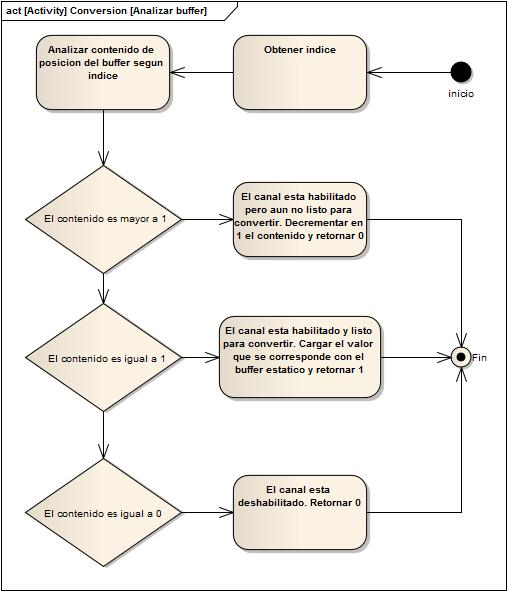
\includegraphics[width=0.80\textwidth, height = 7cm]{actividadanalizarbuffer}
  \caption{Diagrama de actividad que muestra el funcionamiento de la funcion analizar buffer. Esta funcion esta pensada para trabajar junto con "cambiar\_pin". En cada cambio de pin, se analiza el buffer para saber si hay que convertir o no, y actualizar el estado de los elementos del buffer, que corresponden en uno a uno con todas las vias de conversion posibles.}\label{fig:actividadanalizarbuffer}
\end{figure}


 % subsubsection descripcion_de_funcion_analizar\_buffer (end) 

\subsubsection{Descripcion de funcion: cambiar\_pin} % (fold)
\label{ssub:descripcion_de_funcion_cambiar_pin}

\begin{figure}[h]
  \centering
  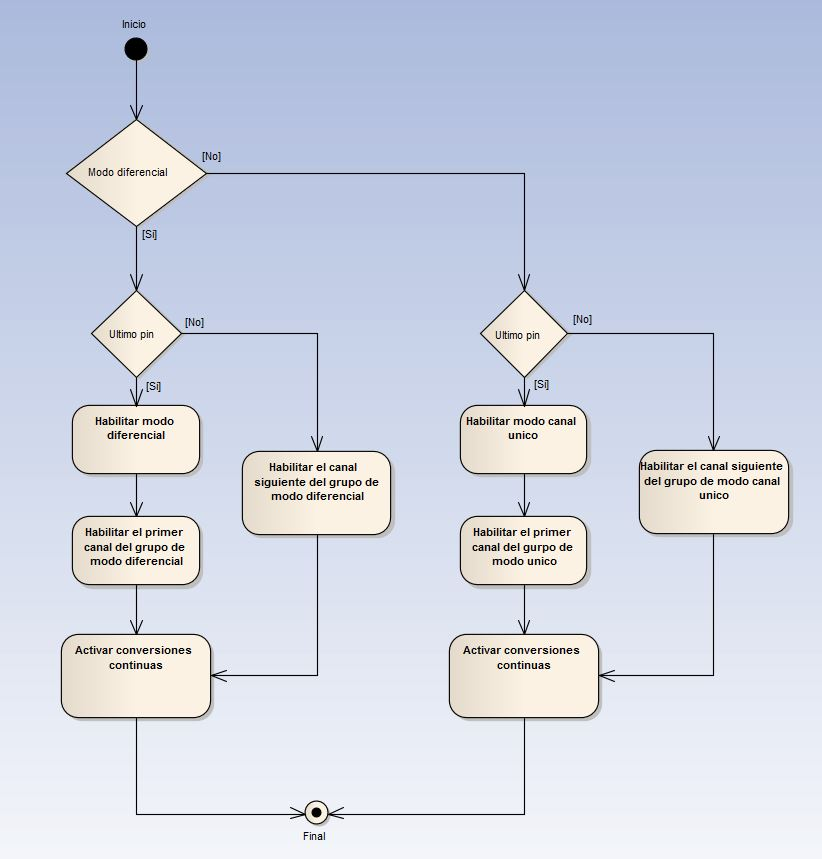
\includegraphics[width=0.80\textwidth, height = 7cm]{actividadcambiarpin}
  \caption[Diagrama de actividad de la funcion cambiar pin]{Diagrama de actividad que ilustra la logica dentro de la funcion cambiar\_pin, dentro del modulo del conversor. Esta funcion es llamada luego de cada conversion. En cada llamado, se selecciona un nuevo canal a medir. No discrimina si el canal esta o no habilitado para medir, en caso en que no lo este, se llamara inmediatamente para cambiar el pin nuevamente sin realizar medicion alguna.}\label{fig:actividadcambiarpin}
\end{figure}

\subsection{Interfaz de usuario} % (fold)
\label{sub:interfaz_de_usuario}

La interfaz de usuario siguio un diseño parecido al terminado en la iteteracion \ref{iteracion_2}. Agregarle funcionailidades es simple gracias al estilo del menu. Cada vez que exista una funcionalidad nueva, hay que conformar un nuevo comando e incluirlo en el espacio de nombres dentro de la interfaz

% subsection interfaz_de_usuario (end)

% subsubsection descripcion_de_funcion_cambiar\_pin (end)

% subsection logica_para_permitir_intervalos_individuales_de_medicion_buffer_de_conversion_estatico_y_dinamico (end)

% section desarrollo (end)

\section{Pruebas} % (fold)
\label{sec:pruebas}

% section pruebas (end)

\section{Resultados} % (fold)
\label{sec:resultados}

% section resultados (end)

% chapter iteracion_5 (end)